% !TEX TS-program = pdflatex
% !TEX encoding = UTF-8 Unicode


\documentclass[11pt]{article} % use larger type; default would be 10pt

\usepackage[utf8]{inputenc} % set input encoding (not needed with XeLaTeX)
\usepackage[portuges]{babel}


%%% PAGE DIMENSIONS
\usepackage{a4}

\usepackage{graphicx} % support the \includegraphics command and options

%%% PACKAGES
\usepackage{booktabs} % for much better looking tables
\usepackage{array} % for better arrays (eg matrices) in maths
\usepackage{paralist} % very flexible & customisable lists (eg. enumerate/itemize, etc.)
\usepackage{verbatim} % adds environment for commenting out blocks of text & for better verbatim
\usepackage{subfig} % make it possible to include more than one captioned figure/table in a single float
% These packages are all incorporated in the memoir class to one degree or another...

%%% HEADERS & FOOTERS
\usepackage{fancyhdr} % This should be set AFTER setting up the page geometry
\pagestyle{fancy} % options: empty , plain , fancy
\renewcommand{\headrulewidth}{0pt} % customise the layout...
\lhead{}\chead{}\rhead{}
\lfoot{}\cfoot{\thepage}\rfoot{}

%%% SECTION TITLE APPEARANCE
\usepackage{sectsty}
\allsectionsfont{\sffamily\mdseries\upshape} % (See the fntguide.pdf for font help)
% (This matches ConTeXt defaults)

%%% ToC (table of contents) APPEARANCE
\usepackage[nottoc,notlof,notlot]{tocbibind} % Put the bibliography in the ToC
\usepackage[titles,subfigure]{tocloft} % Alter the style of the Table of Contents
\renewcommand{\cftsecfont}{\rmfamily\mdseries\upshape}
\renewcommand{\cftsecpagefont}{\rmfamily\mdseries\upshape} % No bold!

%%% END Article customizations

%%% The "real" document content comes below...

\title{Projeto de DSS \\ \large ConfiguraFácil - 1ª Fase}
\date{2018/19}

\begin{document}
\maketitle

\begin{table}[!htbp]
\centering
\begin{tabular}{cc}
 Diogo Sobral (a82523) &  Henrique Pereira (a80261) \\
 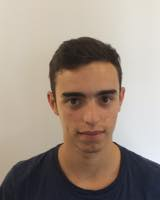
\includegraphics[height=0.8in]{Diogo} &  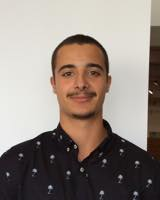
\includegraphics[height=0.8in]{Henrique} \\
	& \\
 Pedro Moreira (a82364)  &   Pedro Ferreira (a81135) \\
 
\includegraphics[height=0.8in]{PedroM} & 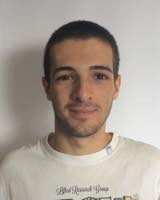
\includegraphics[height=0.8in]{PedroF} \\

\end{tabular}
\end{table}

\newpage
\tableofcontents
\newpage

\section{Introdução}
A primeira fase do projeto da UC Desenvolvimento de Sistemas de Software consiste no desenvolvimento dos modelos de domínio, use cases e da interface com o utilizador para a aplicação ConfiguraFácil. Esta aplicação consiste numa ferramenta existente nos stands de automóveis, que permite junto dos clientes criar uma configuração para uma encomenda de um carro novo. A aplicação guia o cliente em cada fase da configuração, permitindo-lhe escolher componentes individuais ou pacotes pré-definidos. 

Da perspetiva do grupo, a aplicação apresenta os seguintes requisitos:
\begin{itemize}
	\item O cliente pode escolher a pintura, jantes e pneus, motorização e detalhes interiores e exteriores;
	\item O cliente pode também escolher um pacote pré-definido que consiste num agregado de componentes individuais;
	\item Cada componente deve ter uma designação, preço, lista de componentes incompatíveis e lista de componentes complementares;
	\item Sempre que um componente é adicionado à configuração, a aplicação deve verificar se existe alguma incompatibilidade com algum componente previamente selecionado. Se tal existir, o cliente pode optar por desistir da seleção feita ou remover o produto incompatível. Além disso, deve também verificar se é necessário instalar algum componente complementar. Caso aconteça, o cliente pode manter a opção e instalar os componentes necessários ou então desistir da seleção;
	\item Quando um pacote pré-definido é selecionado, devem ser feitas as verificações de dependência/incompatibilidade para cada um dos componentes do pacote;
	\item Deve haver descontos associados aos pacotes, ou seja, os pacotes devem ser mais baratos que a soma os preços individuais de cada um dos seus componentes;
	\item Se o cliente selecionar individualmente todos os componentes que compõem um pacote, a aplicação deve reconhecer tal pacote e aplicar o respetivo desconto;
	\item Após as escolhas básicas, como a pintura e a motorização, o cliente deve poder indicar um orçamento para a encomenda e o sistema deve propor a melhor configuração possível dentro do orçamento apresentado. Ou seja, a aplicação deve conseguir gerar uma configuração ótima dado um orçamento;
	\item Cada componente deve ter um stock associado;
	\item Sempre que chega um novo stock de componentes, o sistema deve conseguir determinar quais são os carros que podem ser produzidos;
	\item Os carros são produzidos por ordem de chegada à fila de configurações efetuadas pelos clientes.
\end{itemize}

\section{Diagrama de Domínio}


\section{Diagrama de Use Cases}

\section{Especificação de Use Cases}

\section{Protótipo de Interface}

\section{Diagrama de Máquinas de Estado}


\end{document}
